\section{Numerical Results}

\begin{frame}
    \begin{center}
        \huge 4.1: \textbf{Numerical Results}\\
        {\normalsize\noindent (Hypersonic Thermal Protection Systems)}
    \end{center}
\end{frame}

%%%%%%%%%%%%%%%%%%%%%%%%%%%%%%%%%%%%%%%%% Hypersonic TPS %%%%%%%%%%%%%%%%%%%%%%%%%%%%%%%%%%%%%%%%%%

\begin{frame}{Numerical Results: Hypersonic Thermal Protection Systems}
    \footnotesize
    \visible<1->{
    Modeling \textbf{hypersonic thermal protection systems} (TPS) is challenging,}
    \begin{columns}
        \visible<3->{
        \begin{column}{0.3\textwidth}
            \begin{graybox}{Full-Order Model}
                \begin{align*}
                    \visible<4->{
                    \dot{\vx} &= \vF\left(\vx;\vp\right)}\\
                    \visible<5->{
                    \vz_{\text{HF}} &= \vH\left(\vx;\vp\right)}\\
                    \visible<6->{
                    \vx(t_0) &= \vx_0}
                \end{align*}
                \vspace{-0.2in}
                \begin{enumerate}
                    \item<4-> $\vx\in\mathbb{R}^{n_x}$: states
                    \item<4-> $\vp\in\mathbb{R}^{n_p}$: parameters
                    \item<5-> $\vz_{\text{HF}}\in\mathbb{R}^{n_z}$: QoI 
                \end{enumerate}
            \end{graybox}
        \end{column}}
        \visible<2->{
        \begin{column}{0.7\textwidth}
            \centering
            \begin{graybox}{Thermal Protection Systems}
                \begin{figure}
                    \centering
                    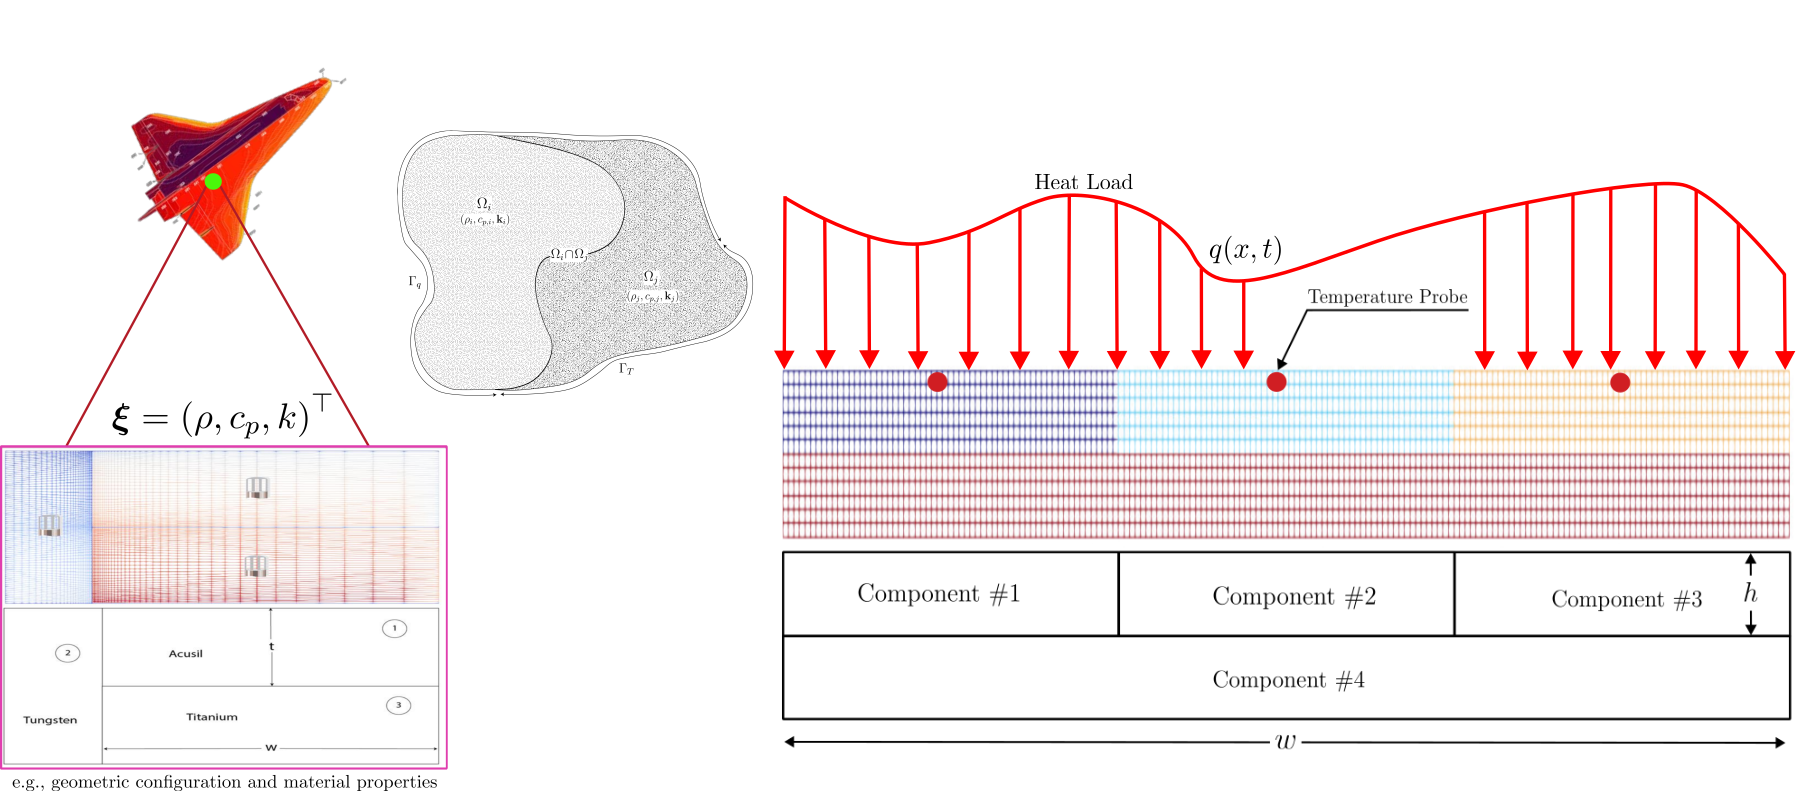
\includegraphics[width=0.9\textwidth]{../figs/ablation/tps.png}
                \end{figure}
                \centering
                Parameters $\vxi$: \textbf{boundary conditions} and \textbf{material properties}
            \end{graybox}
        \end{column}}
    \end{columns} 
\end{frame}

\begin{frame}{Numerical Results: Hypersonic Thermal Protection Systems}
    \footnotesize
    \visible<1->{
    The FOM is \textbf{too costly to evaluate}, thus we apply \textbf{coarse-graining} [2],}
    \visible<2->{
    \begin{figure}
        \centering
        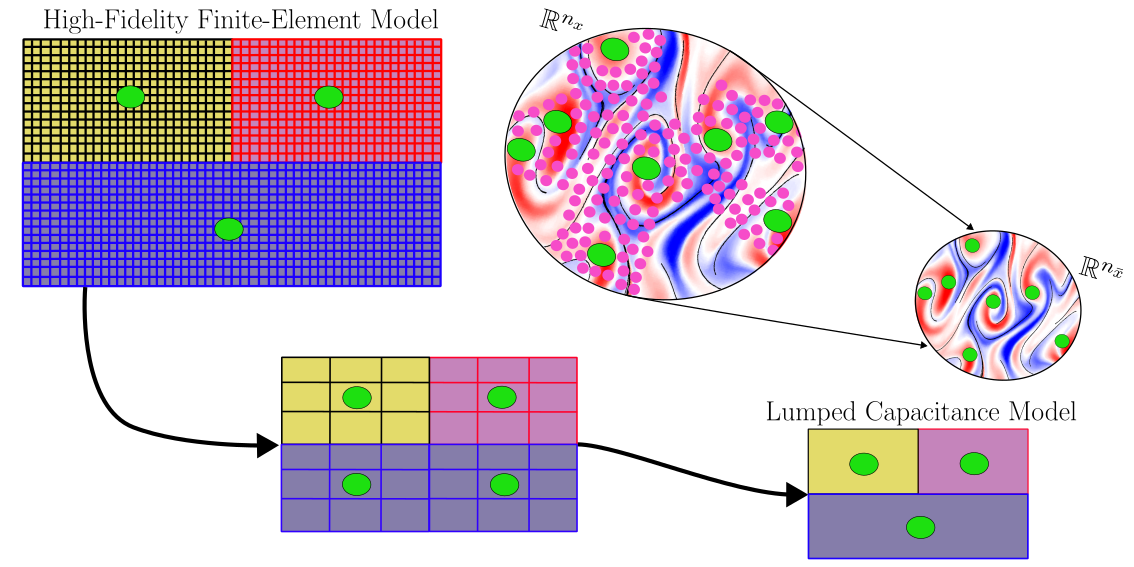
\includegraphics[width=0.8\textwidth]{../figs/ablation/coarse_graining_lcm.png}
    \end{figure}}
\end{frame}

\begin{frame}{Numerical Results: Hypersonic Thermal Protection Systems}
    \footnotesize
    \visible<1->{
    \textbf{Coarse-graining} DG-FEM yields the \textbf{lumped capacitance model},}
    \begin{columns}
        \begin{column}{0.4\textwidth}
            \centering
            \visible<2->{
            \begin{graybox}{Energy Full-Order Model}
                \centering
                \vspace*{-0.1in}
                \begin{equation*}
                    \vA(\vu)\dot{\vu} = \vB(\vu)\vu + \vf(t)
                \end{equation*}
            \end{graybox}}
            \visible<3->{
            \begin{graybox}{Projection Operator}
                \centering
                \vspace*{-0.1in}
                \begin{equation*}
                    \cP: \mathcal{G}(\vu) \mapsto \bar{\mathcal{G}}(\bvu)
                \end{equation*}
            \end{graybox}}
            \visible<4->{
            \begin{graybox}{Lumped Capacitance Model}
                \centering
                \vspace*{-0.1in}
                \begin{equation*}
                    \bar{\vA}(\bvu)\dot{\bvu} = \bar{\vB}(\bvu)\bvu + \bar{\vf}(t)
                \end{equation*}
            \end{graybox}}
        \end{column}
        \visible<5->{
        \begin{column}{0.6\textwidth}
            \centering
            \begin{figure}
                \centering
                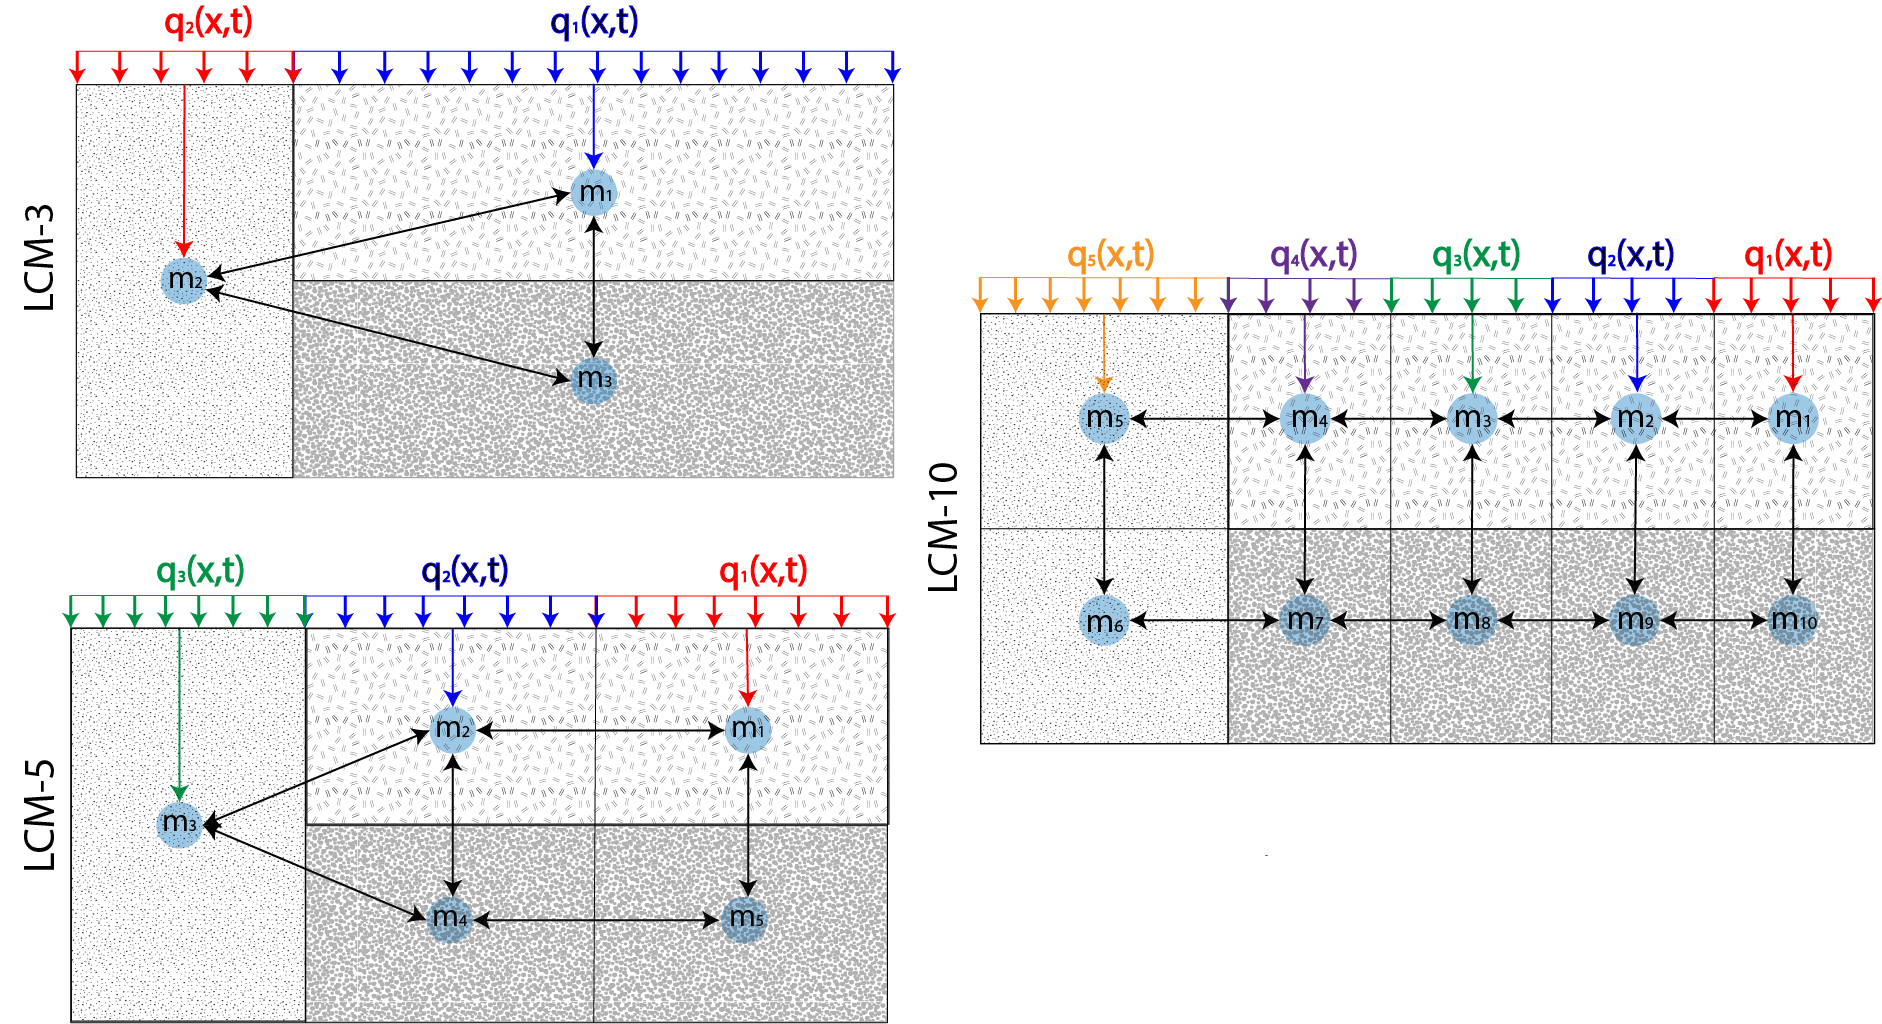
\includegraphics[width=0.95\textwidth]{../figs/tps/lcms.png}
            \end{figure}
        \end{column}}
    \end{columns}
    \begin{center}
        \tiny
        $\vA$: capacitance matrix, $\vB$: conduction matrix, $\bvu$: average temperatures, $\vw$: one-dimensional surface recession, $\vXi$: recession-rate matrix, $\hat{\vf}$: recession forcing, $\bar{\vf}$: heat flux forcing.
    \end{center}
\end{frame}

\begin{frame}{Numerical Results: Hypersonic Thermal Protection Systems}
    \footnotesize
    \visible<1->{Physics infusion is performed using the following \textbf{memory kernel} approximation,}
    \visible<2->{
    \begin{graybox}{Physics-Infused ROM}
        \visible<3->{
        Memory kernel approximation,
        \vspace{-0.1in}
        \begin{equation*}
            \vkappa(t,s,\bvu) \approx \sum_{j=1}^{m} e^{-\lambda_j(t-s)}\vp_j\left(\vq_j^\top\bvu(s) + \vr_j^\top\bar{\vf}(s)\right)
            \vspace*{-0.2in}
        \end{equation*}}
        \visible<4->{
        Markovian reformulation yields,}
        \begin{align*}
            \visible<5->{
            \bar{\vA}(\bvu)\dot{\bvu} &= \bar{\vB}(\bvu)\bvu + \bar{\vf} + \textcolor{red}{\vP}\vbeta\quad\rightarrow\text{physics-infused LCM}}\\
            \visible<6->{
            \dot{\vbeta} &= \textcolor{red}{\vQ} - \textcolor{red}{\vLambda}\vbeta + \textcolor{red}{\vR}\bar{\vf}(t)\quad\rightarrow\text{hidden dynamics (DG-FEM form)}}\\
            \visible<7->{
            \vz &= \textcolor{red}{\vD}\vy\quad\rightarrow\text{temperature probe output}}
        \end{align*}
    \end{graybox}}
    \vspace*{-0.1in}
    \begin{columns}
        \begin{column}{0.5\textwidth}
            \visible<8->{
            \begin{graybox}{Learnable Parameters}
                \centering
                \begin{equation*}
                    \redvTheta = \left\{\textcolor{red}{\vP}, \textcolor{red}{\vQ}, \textcolor{red}{\vLambda}, \textcolor{red}{\vR}, \textcolor{red}{\vD}\right\}\in\mathbb{R}^{n_\theta}
                \end{equation*}
                \textbf{Need to identify these from data!}
            \end{graybox}}
        \end{column}
        \begin{column}{0.5\textwidth}
            \visible<9->{
            \begin{graybox}{Physics-Infused ROM}
                \begin{align*}
                    \vzero &= \vcD\left(\dot{\vy},\vy,\vp;\redvTheta\right)\\
                    \vz &= \textcolor{red}{\vD}\vy
                \end{align*}
            \end{graybox}}
        \end{column}
    \end{columns}
\end{frame}

\begin{frame}{Numerical Results: Hypersonic Thermal Protection Systems}
    \footnotesize
    \begin{center}
        \visible<1->{
        \begin{graybox}{Parametrization}
            \centering
            \visible<2->{
            \textbf{boundary conditions}: $\vxi_{\text{BC}} = \left[\xi_0,\xi_1,\xi_2\right]^\top$,} \visible<3->{\textbf{material properties}: $\vxi_{\text{M}} = \left[\alpha_0,\alpha_1,\alpha_2\right]^\top$}
            \begin{equation*}
                \visible<2->{
                q(x,t;\vxi_{\text{BC}}) = q_1(x;\vxi_{\text{BC}})q_2(t;\vxi_{\text{BC}})},\quad \visible<3->{m(T;\vxi_{\text{M}}) = m^{(n)}(T) + m^{(p)}(T;\vxi_{\text{M}})}
                \vspace*{-0.1in}
            \end{equation*}
            \vspace*{-0.1in}
        \end{graybox}}
    \end{center}
    \vspace*{-0.2in}
    \begin{columns}
        \begin{column}{0.5\textwidth}
            \visible<4->{
            \begin{graybox}{Parameter Space}
                \begin{figure}
                    \centering
                    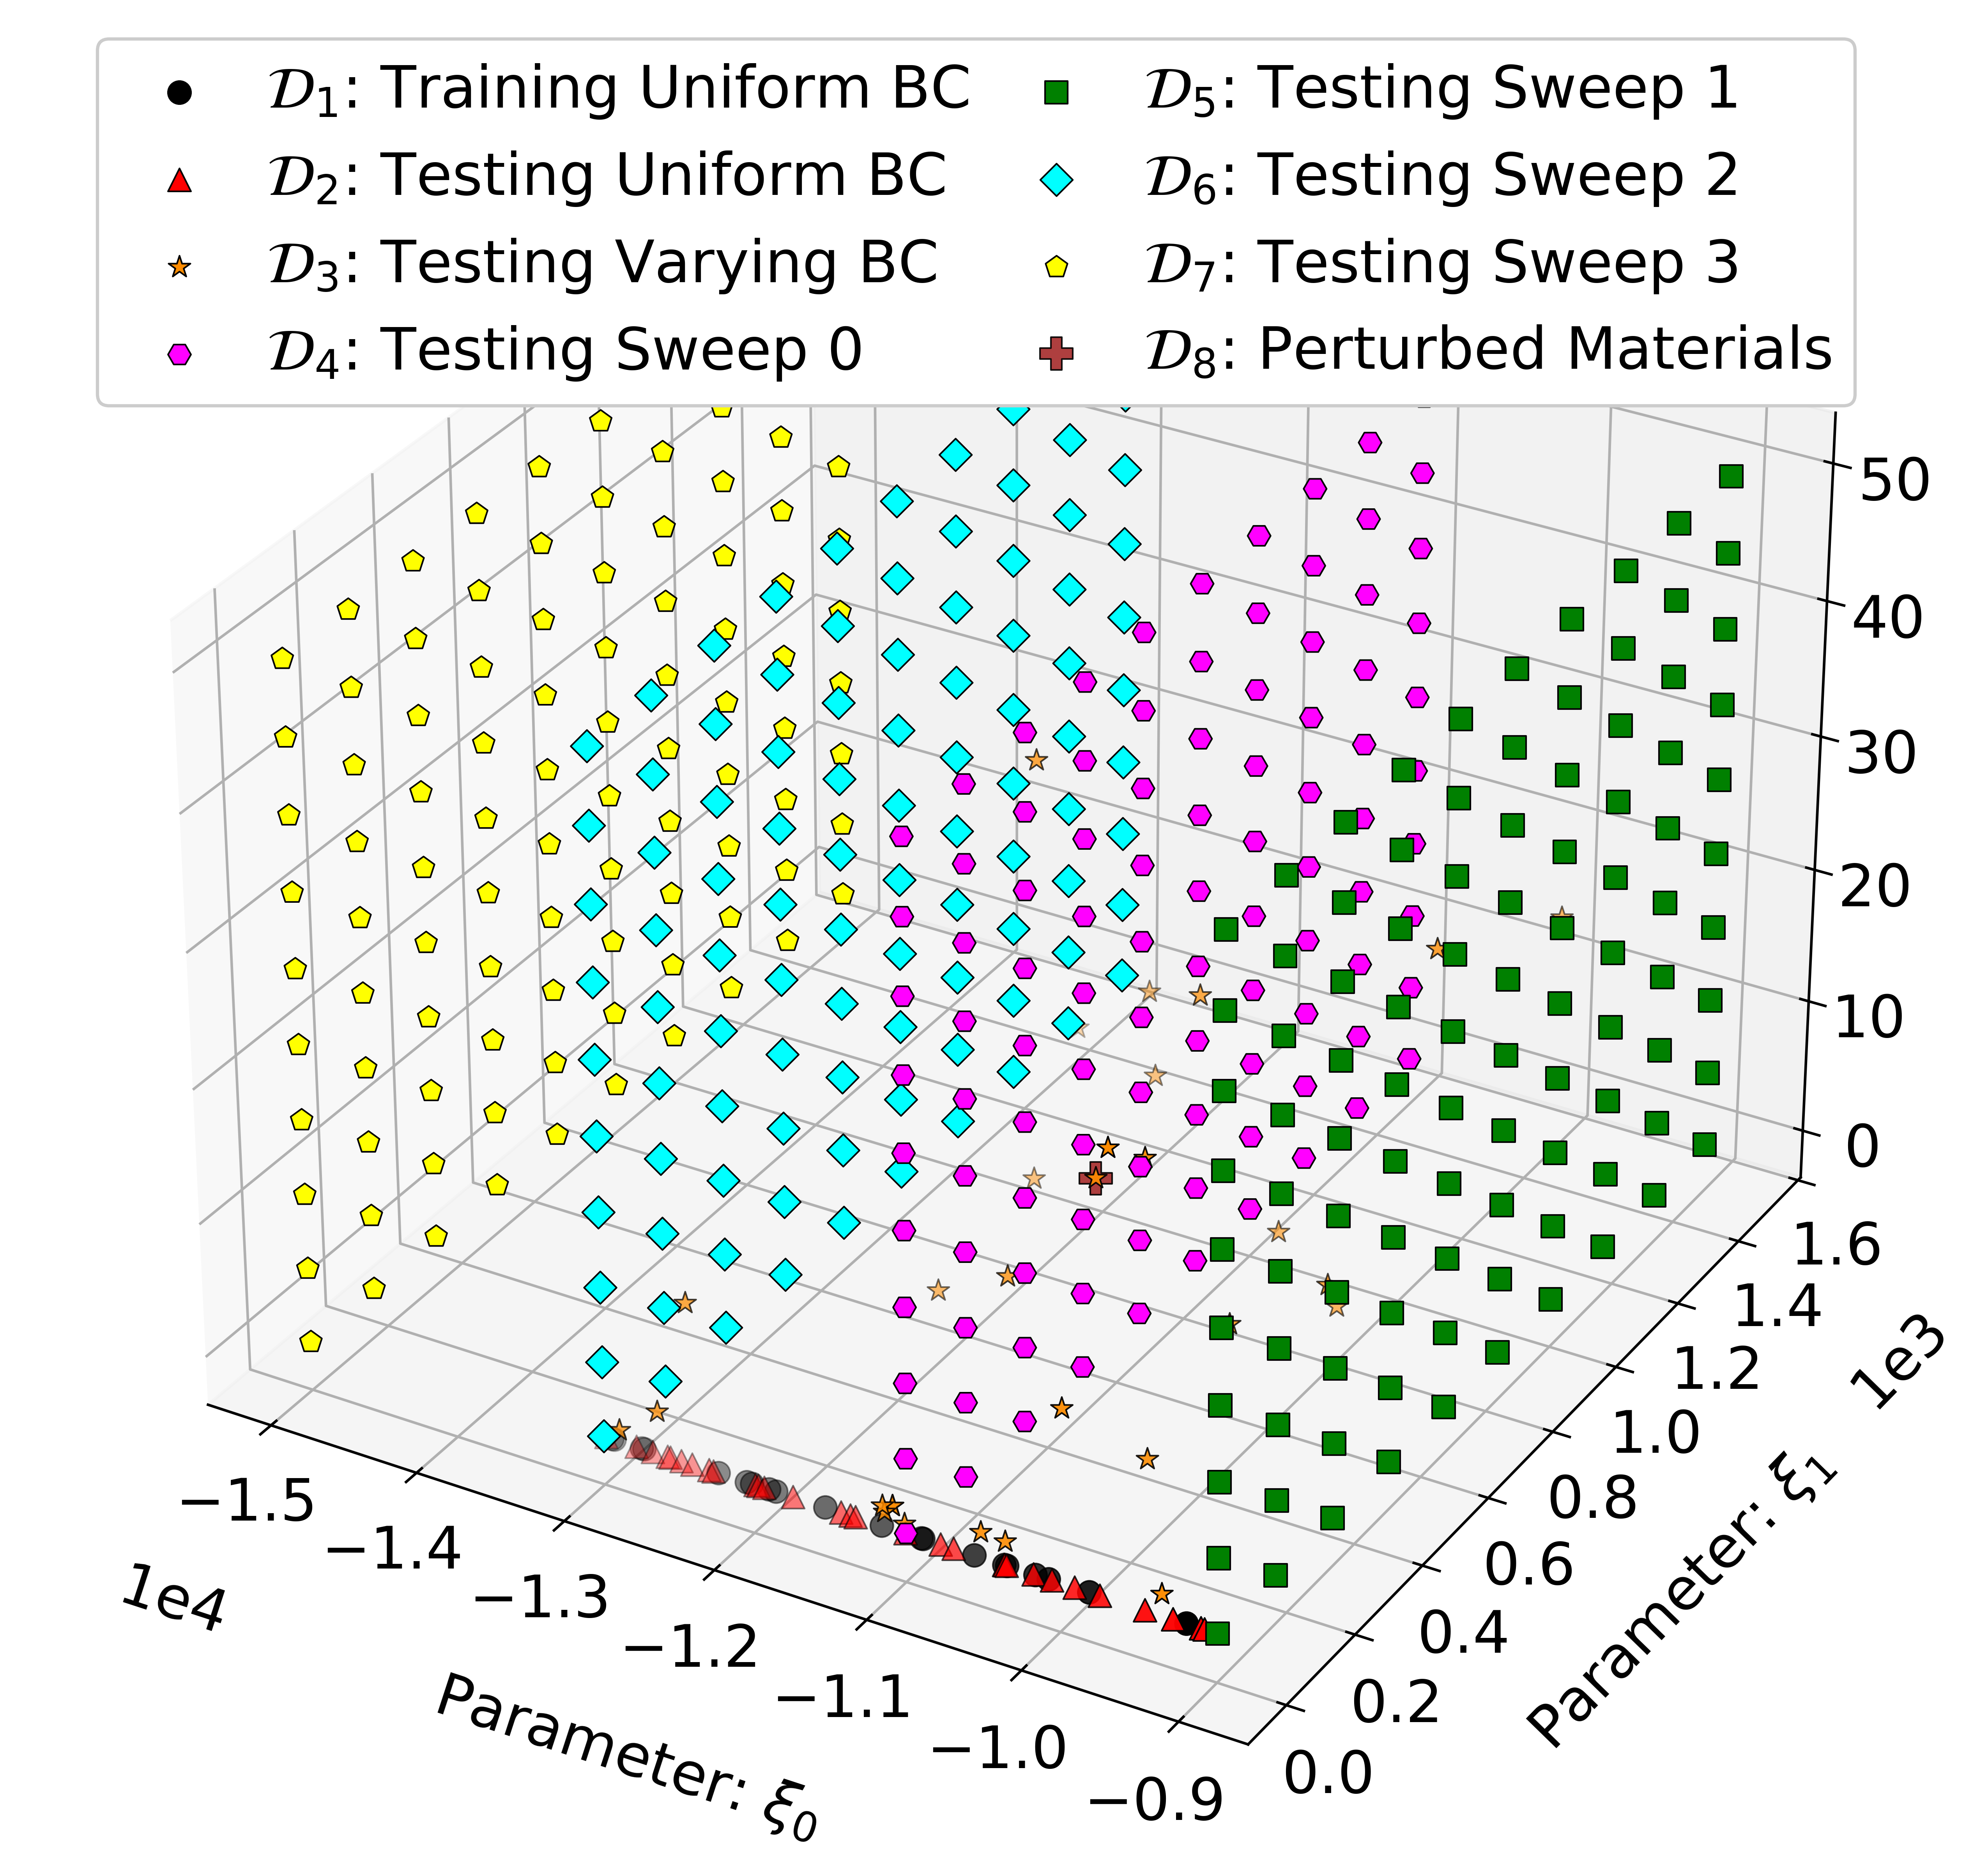
\includegraphics[width=0.6\textwidth]{../figs/tps/samples.png}
                \end{figure}
            \end{graybox}}
        \end{column}
        \begin{column}{0.5\textwidth}
            \visible<5->{
            \begin{graybox}{High-Fidelity Observables}
                \only<5>{
                    \begin{figure}
                        \centering
                        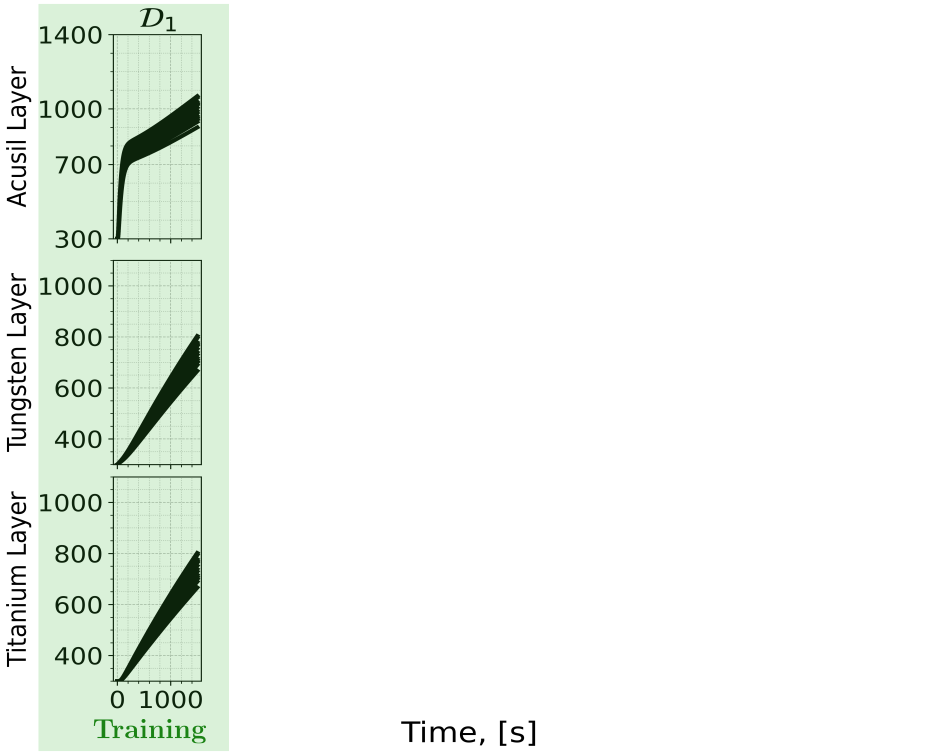
\includegraphics[width=0.9\textwidth]{../figs/tps/tps_data_1.png}
                    \end{figure}}
                \only<6>{
                    \begin{figure}
                        \centering
                        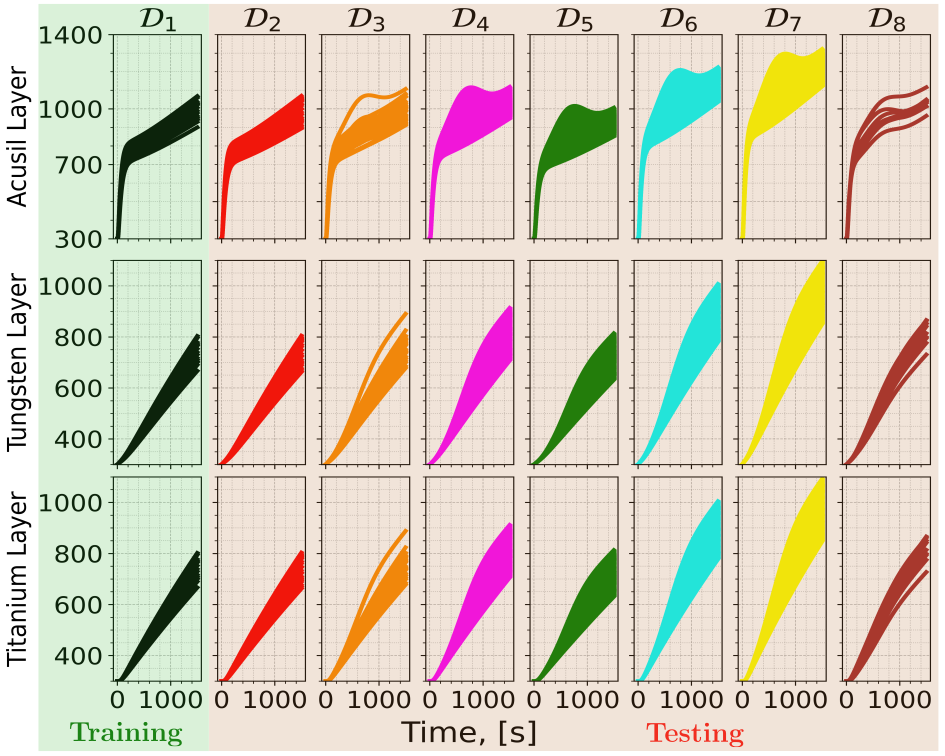
\includegraphics[width=0.9\textwidth]{../figs/tps/tps_data_2.png}
                    \end{figure}}
            \end{graybox}}
        \end{column}
    \end{columns}
\end{frame}

\begin{frame}{Numerical Results: Hypersonic Thermal Protection Systems}
    \footnotesize
    \visible<1->{\textbf{Quantify} the impossible trinity of modeling (ITM),}
    \begin{columns}
        \visible<2->{
        \begin{column}{0.4\textwidth}
            \begin{figure}
                \centering
                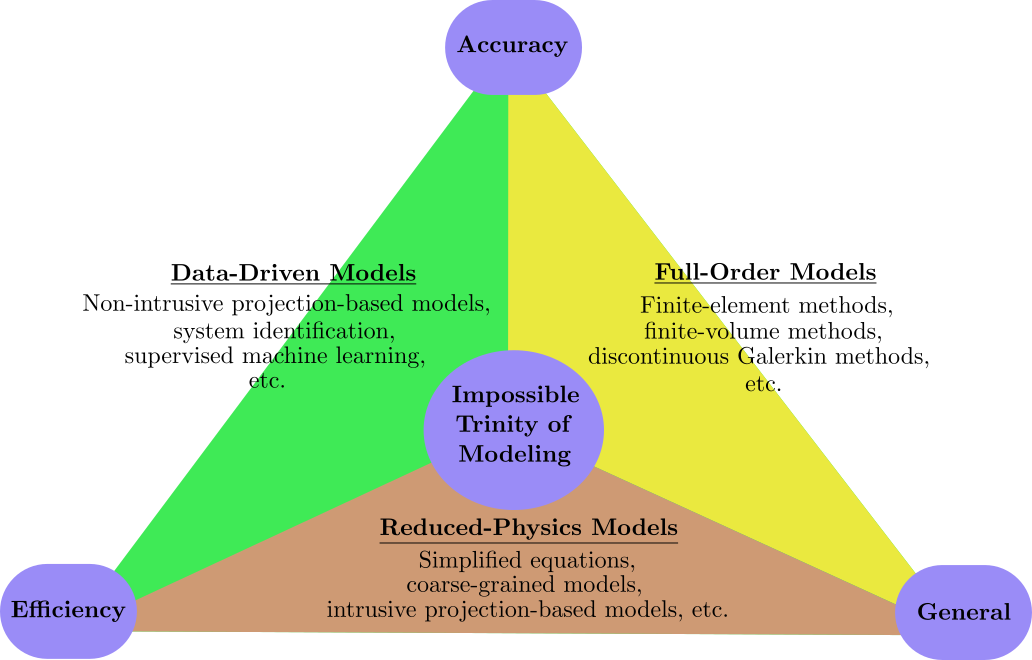
\includegraphics[width=0.9\textwidth]{../figs/introduction/itm.png}
            \end{figure}}
        \end{column}
        \begin{column}{0.6\textwidth}
            \centering
            \begin{itemize}
                \visible<3->{
                \item \textbf{Accuracy}: normalized root mean square error (NRMSE),
                \begin{equation*}
                    e_i^{(l)} = \frac{1}{\Delta z_{i,\text{HF}}^{(l)}}\sqrt{\frac{1}{p}\sum_{k=0}^{p-1}\left(z_{i,\text{HF}}^{(l)}(t_k) - z_{i,\text{ROM}}^{(l)}(t_k)\right)^2}, \quad i=u,w
                \end{equation*}}
                \visible<4->{
                \item \textbf{Efficiency}: computational acceleration factor,
                \begin{equation*}
                    \frac{\mathcal{T}_{\text{HF}}(\mathcal{D})}{\mathcal{T}_{\text{ROM}}(\mathcal{D})}
                \end{equation*}}
                \visible<5->{
                \item \textbf{Generalizability}: accuracy for unseen BCs and SRMs,
                \begin{equation*}
                    \text{(\textcolor{red}{difficult for ROMs with sparse training data!})}
                \end{equation*}}
            \end{itemize}
        \end{column}
    \end{columns}
    \vspace{-0.1in}
    \begin{center}
        \tiny $\mathcal{T}_{\text{HF}}$: FOM wall-clock time, $\mathcal{T}_{\text{ROM}}$: ROM wall-clock time, $\Delta z_{i,\text{HF}}^{(l)}$: range of HF observables in trajectory $l$, $p$: number of time points, $\mathcal{D}$: dataset
    \end{center}
\end{frame}

\begin{frame}{{Numerical Results: Hypersonic Thermal Protection Systems}}
    \footnotesize
    \visible<1->{Performance of PIROM vs \textbf{SoTA SciML methods}},
    \begin{columns}
        \begin{column}{0.45\textwidth}
            \visible<2->{
            \begin{graybox}{Observable Prediction}
                \begin{figure}
                    \centering
                    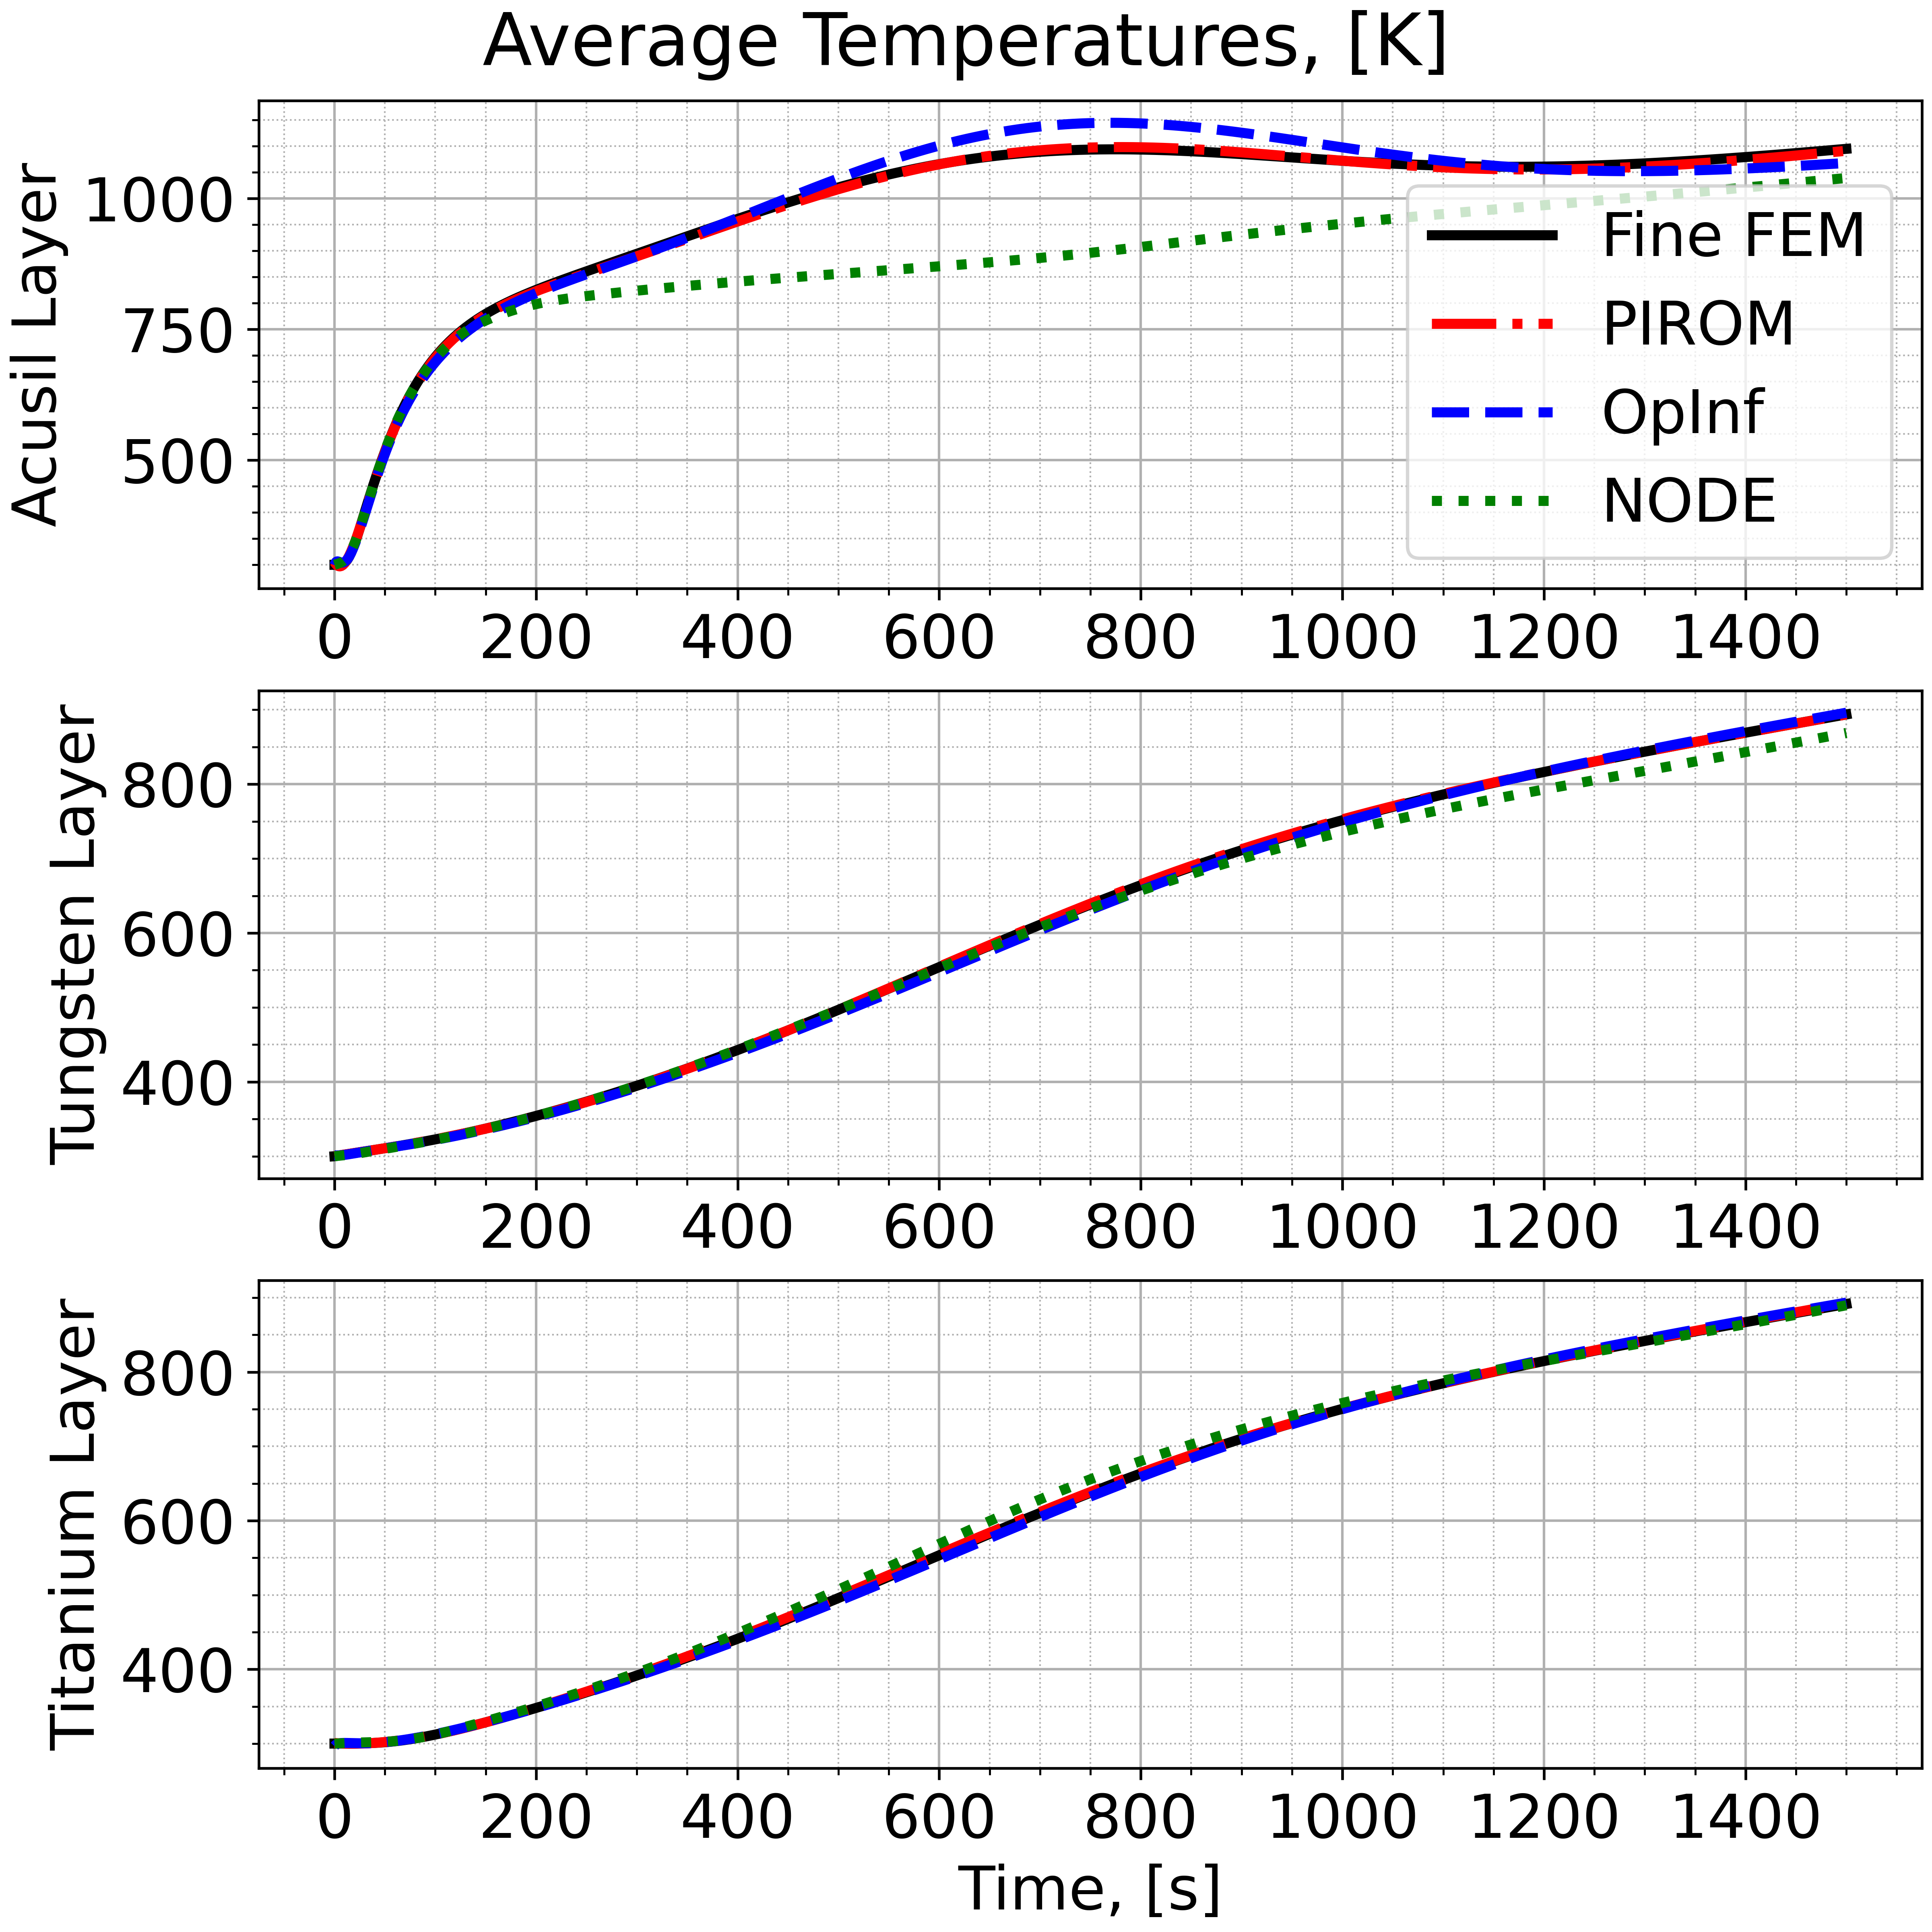
\includegraphics[width=0.9\textwidth]{../figs/tps/pirom_vs_opinf_vs_node_test_varying_sweep_0_case_95.png}
                \end{figure}
            \end{graybox}}
        \end{column}
        \hspace*{-0.1in}
        \begin{column}{0.6\textwidth}
            \visible<3->{
            \begin{graybox}{PIROM vs OpInf vs NODE}
                \centering
                \begin{figure}
                    \centering
                    \includegraphics[width=0.9\textwidth]{../figs/tps/pirom_vs_opinf_vs_node_varying_sweep_0_varying_materials.png}
                \end{figure}
            \end{graybox}}
        \end{column}
    \end{columns}
    \begin{center}
        {\tiny FEM: finite-element method, NODE: neural ordinary differential equations, OpInf: operator inference, NRMSE: normalized root mean square error
        }
    \end{center}
\end{frame}

\begin{frame}{Numerical Results: Hypersonic Thermal Protection Systems}
    \footnotesize
    \visible<1->{Performance of PIROM vs \textbf{SoTA SciML methods},}
    \begin{columns}
        \begin{column}{0.5\textwidth}
            \visible<1->{
            \begin{graybox}{Accuracy/Generalizability Comparison}
                \begin{figure}
                    \centering
                    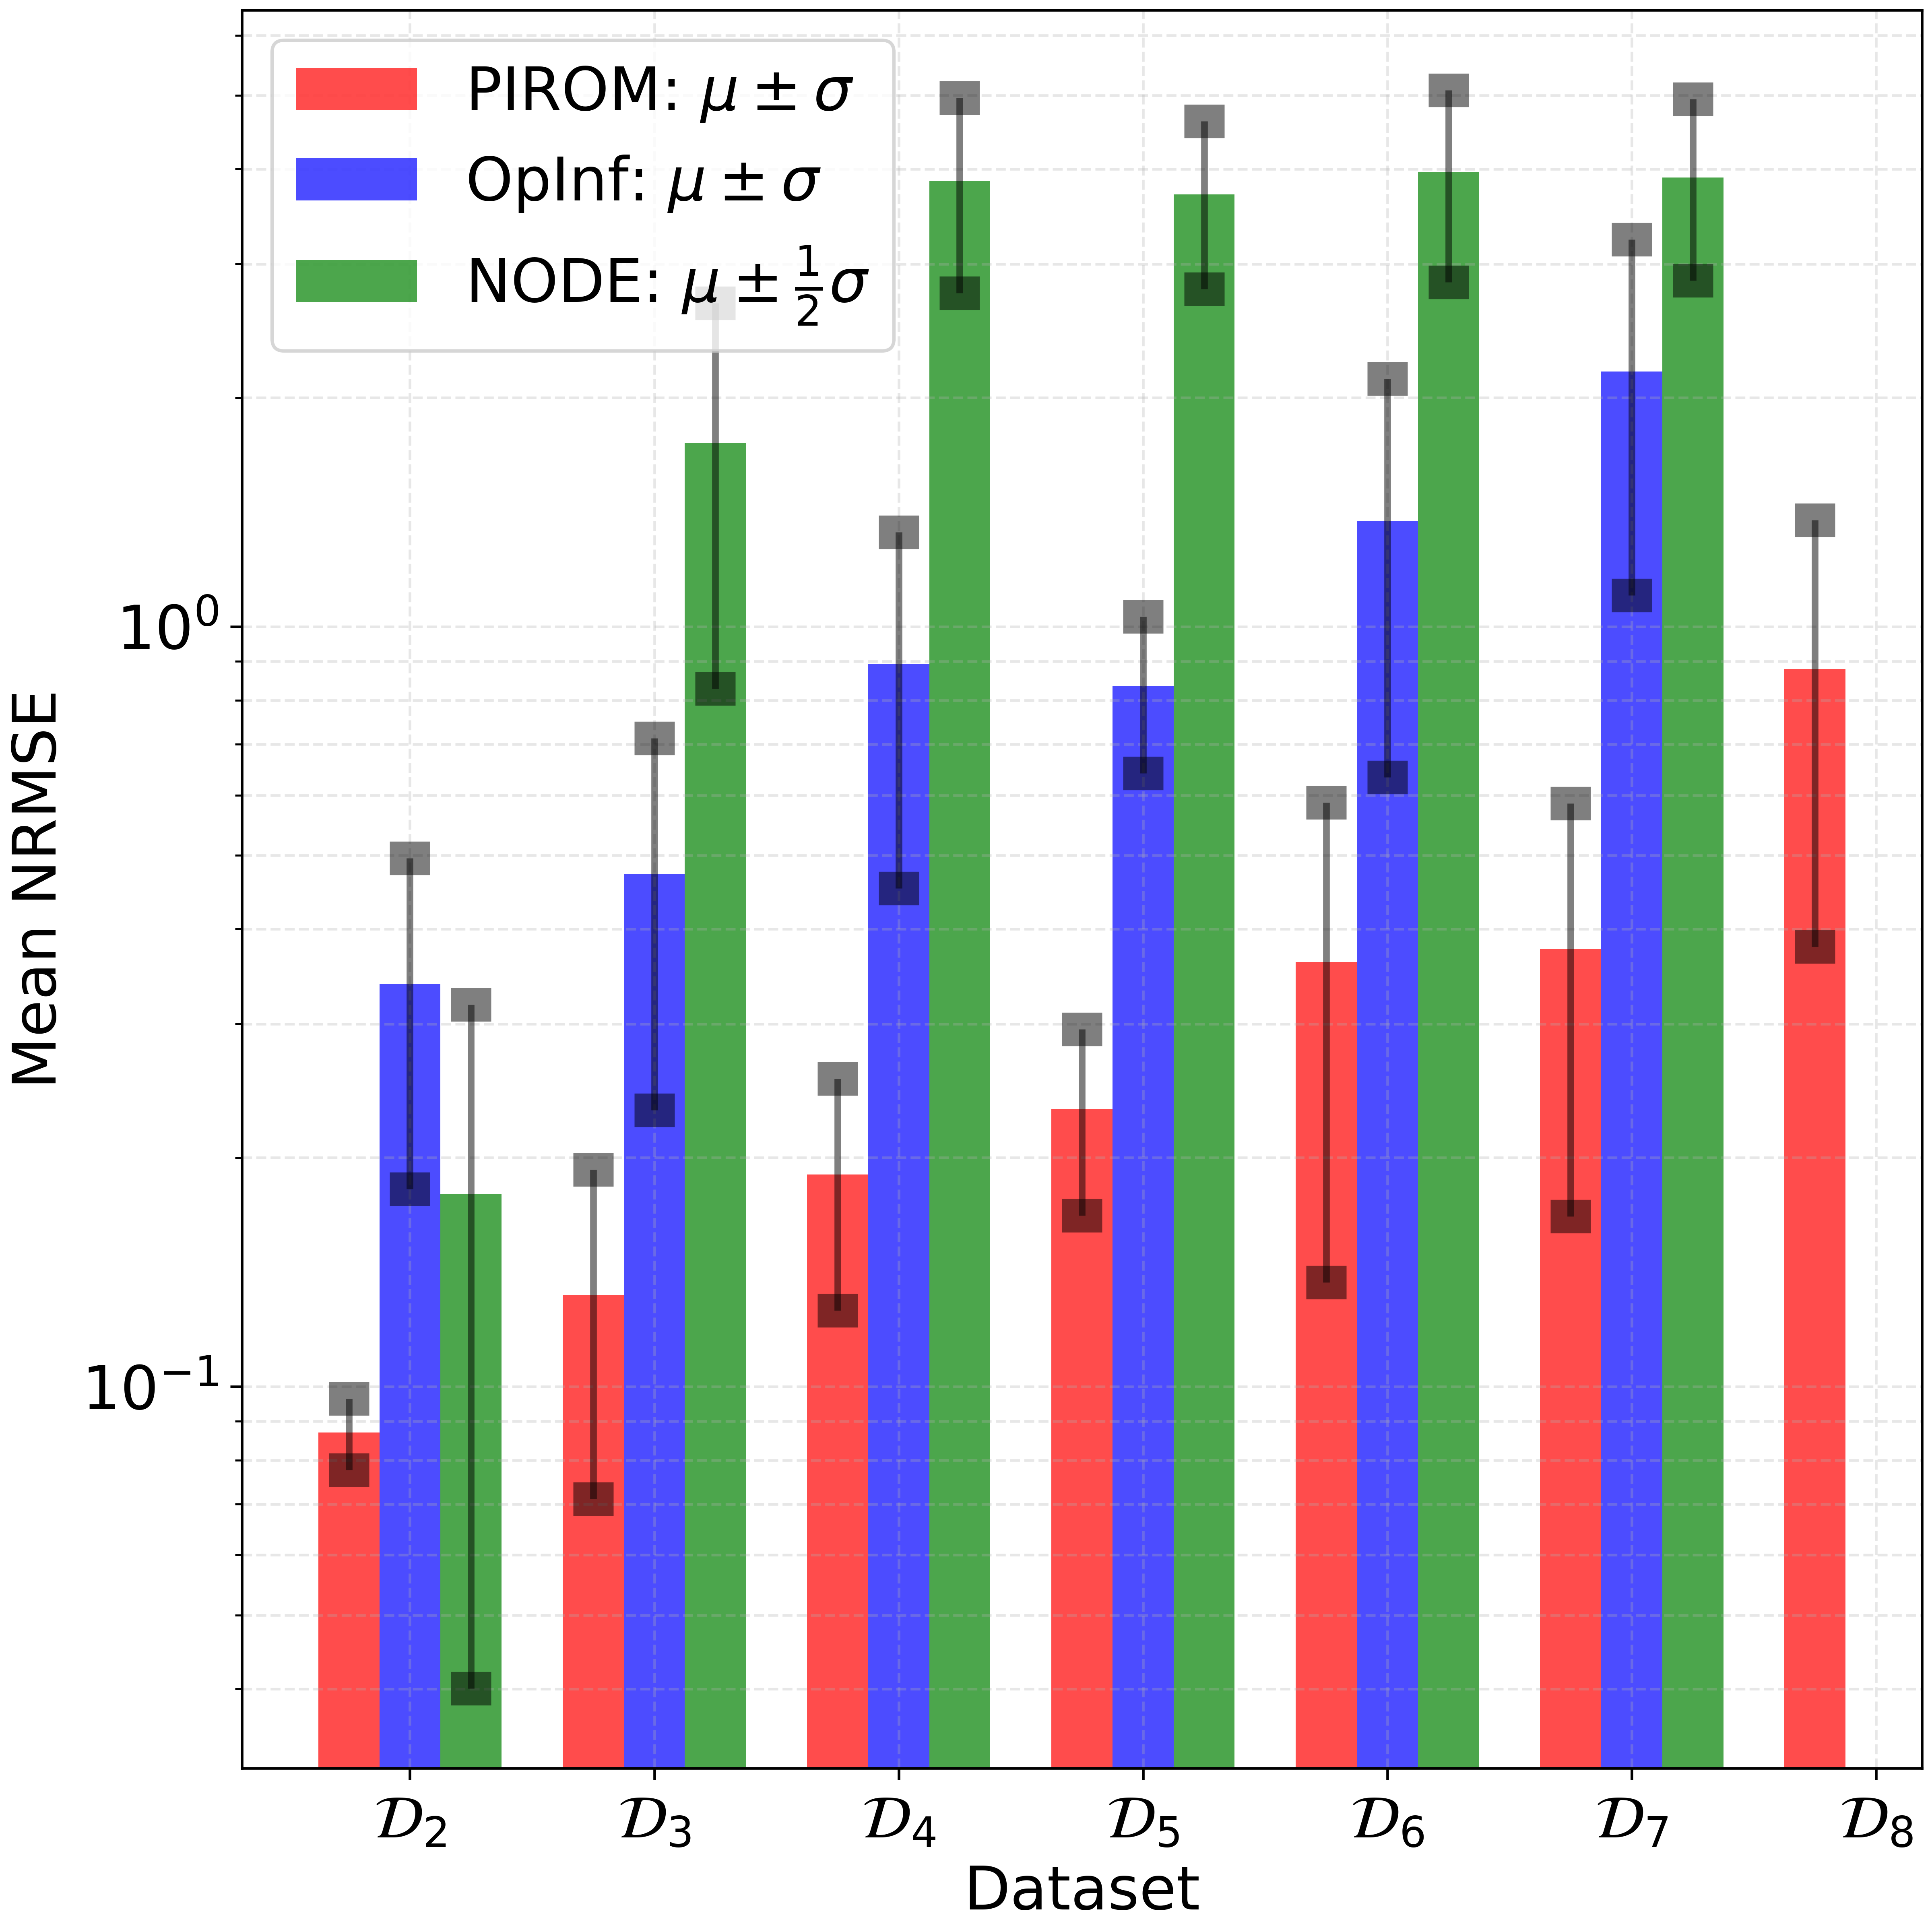
\includegraphics[width=0.80\textwidth]{../figs/tps/model_nrmses_bar_plot.png}
                \end{figure}
            \end{graybox}}
        \end{column}
        \begin{column}{0.5\textwidth}
            \visible<2->{
            \begin{graybox}{Computational Efficiency}
                \begin{figure}
                    \centering
                    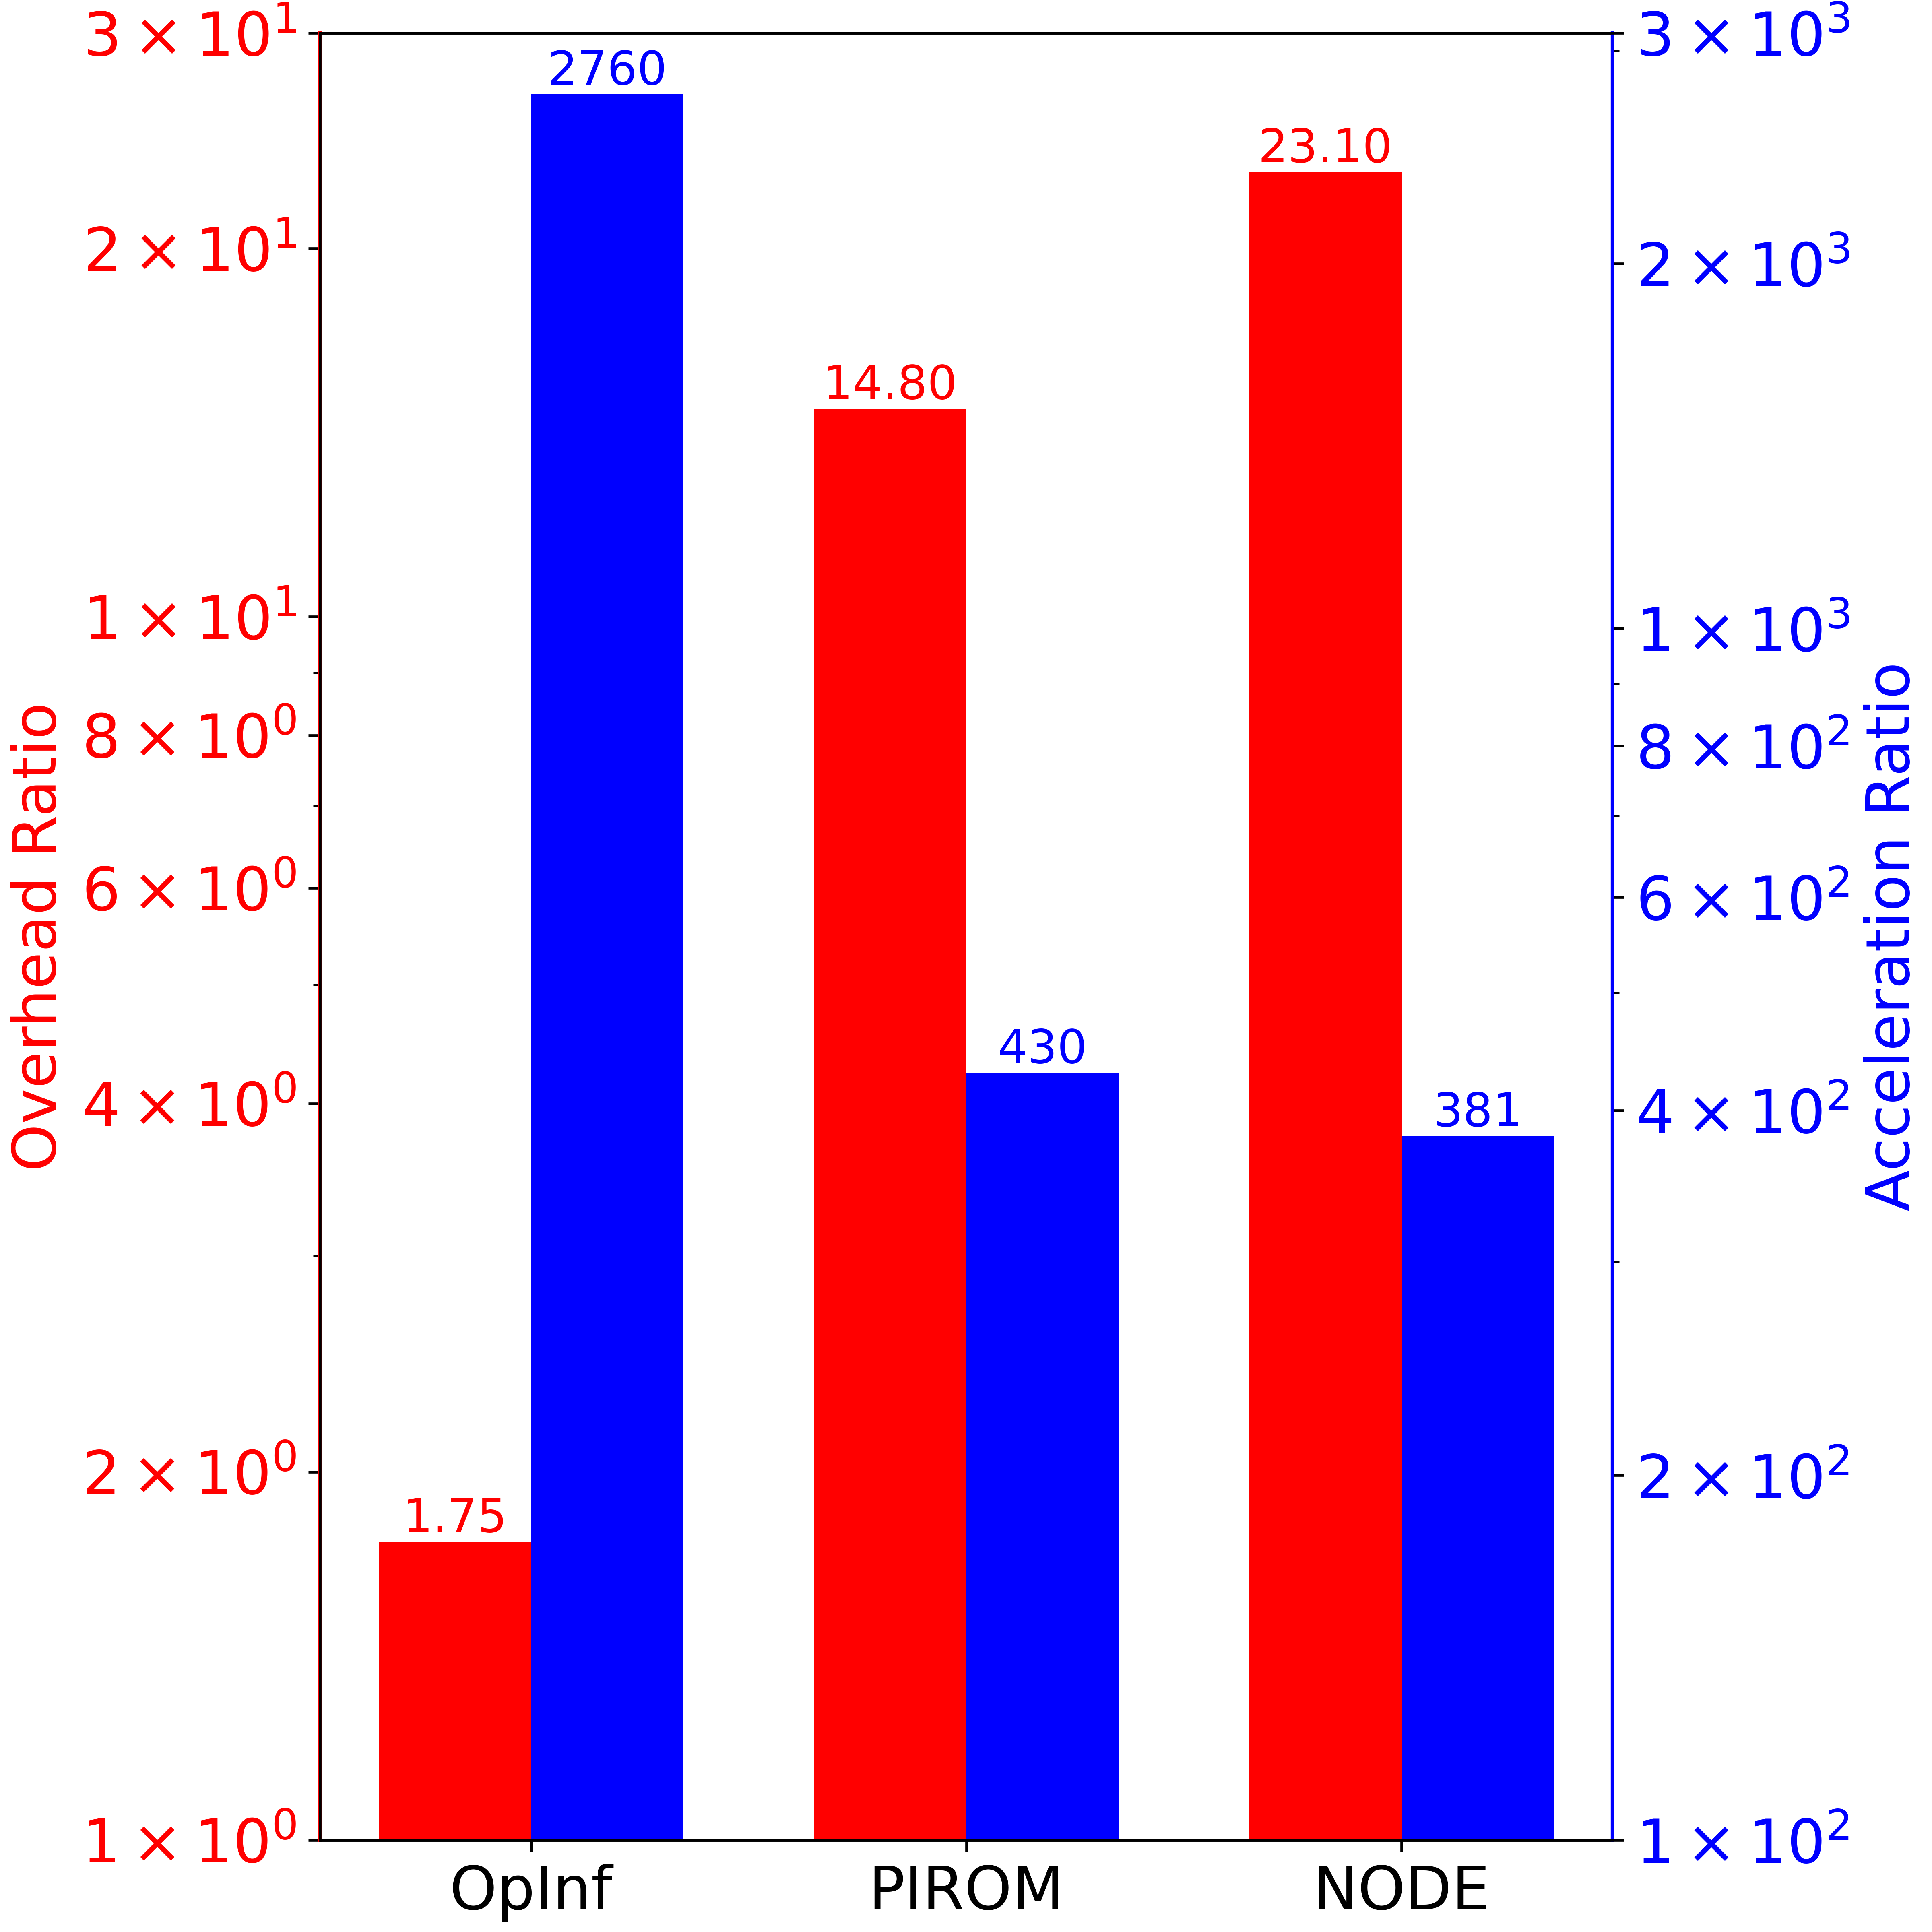
\includegraphics[width=0.80\textwidth]{../figs/tps/ratios.png}
                \end{figure}
            \end{graybox}}
        \end{column}
    \end{columns}
    \visible<1->{
    \begin{center}
        {\tiny FEM: finite-element method, NODE: neural ordinary differential equations, OpInf: operator inference, NRMSE: normalized root mean square error}
    \end{center}}
\end{frame}

\begin{frame}{Numerical Results: Hypersonic Thermal Protection Systems}
    \footnotesize
    \begin{columns}
        \visible<2->{
        \begin{column}{0.4\textwidth}
            \centering
            \textbf{Is the ITM solved?}
            \begin{figure}
                \centering
                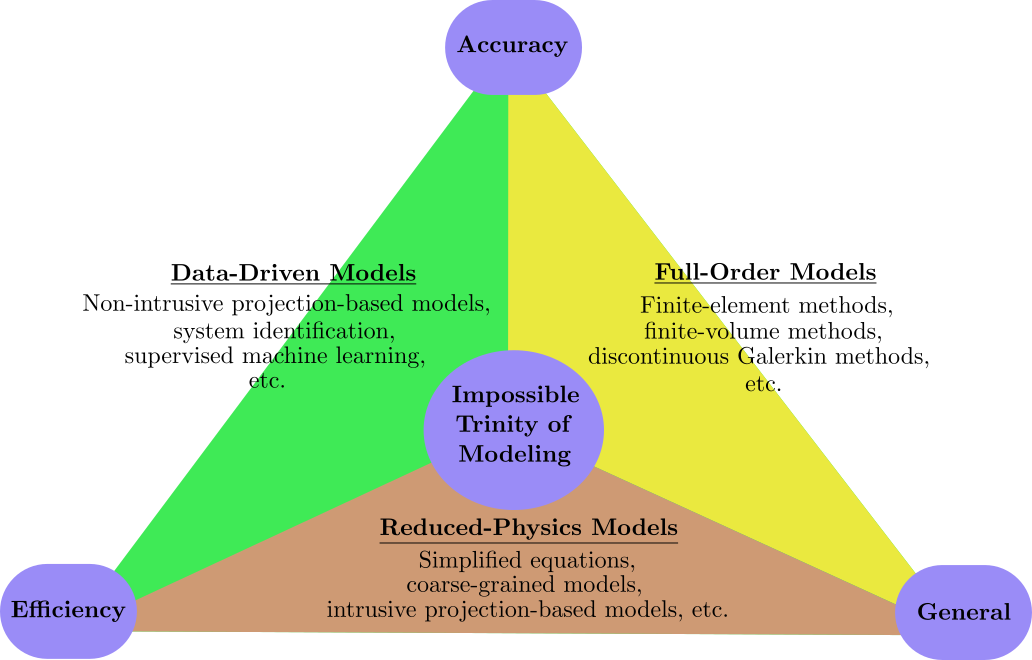
\includegraphics[width=0.9\textwidth]{../figs/introduction/itm.png}
            \end{figure}
        \end{column}}
        \begin{column}{0.7\textwidth}
            \centering
            \begin{itemize}
                \item<3-> \textbf{Accuracy}: comparable to FOMs (NRMSE $<1\%$),
                \item<4-> \textbf{Efficiency}:
                \begin{itemize}
                    \item<5-> \textcolor{red}{\textbf{Training}}: similar to NODE, but slower than OpInf
                    \item<6-> \textcolor{blue}{\textbf{Evaluation}}: similar to NODE, but ``slower'' than OpInf
                \end{itemize}
                \item<7-> \textbf{Generalizability}:
                \begin{itemize}
                    \item<8-> \textbf{Dimensions}: un-seen loading conditions,
                    \item<9-> \textbf{Physics}: un-seen material properties 
                \end{itemize}
            \end{itemize}
        \end{column}
    \end{columns}
    \visible<3->{
    \begin{tikzpicture}[remember picture, overlay]
        \node[anchor=north west, xshift=2.29cm, yshift=-2.8cm] at (current page.north west) {
\includegraphics[width=0.1\textwidth]{../figs/pirom/checkmark.png}};
    \end{tikzpicture}}
    \visible<4->{
    \begin{tikzpicture}[remember picture, overlay]
        \node[anchor=north west, xshift=0.1cm, yshift=-5.8cm] at (current page.north west) {
\includegraphics[width=0.08\textwidth]{../figs/pirom/exclamation.png}};
    \end{tikzpicture}}
    \visible<5->{
    \begin{tikzpicture}[remember picture, overlay]
        \node[anchor=north west, xshift=4.45cm, yshift=-5.6cm] at (current page.north west) {
\includegraphics[width=0.1\textwidth]{../figs/pirom/checkmark.png}};
    \end{tikzpicture}}
\end{frame}

